\section{Discussion} \label{sec:discussion}

\subsection{Comparison to baseline approach}
Our baseline approach was the Delta Method described in Section
\ref{subsec:method:delta_method}. One of the goals of this report was finding
and implementing methods for authorship verification that could beat our
baseline method. An overview of the different methods final results can be seen
in Table \ref{tab:all_final_results}. It can be seen that we were able to beat
the baseline method both on the PAN 2013 dataset and the PAN 2015 dataset.

% TODO: Maybe elaborate on what it means that we beat the baseline methods.

\begin{table}
    \centering
    \begin{tabular}{|c|c|c|c|}
    \hline
    \textbf{Method}             & \textbf{P2013.1 F1 Score} & \textbf{P2013.2 F1 Score} & \textbf{P2015 Final Score} \\ \hline
    Delta (BASELINE)            & 0.64438                      & 0.63291                      & 0.3188                        \\ \hline
    Random Forest (\gls{UBM}) & -                            & -                            & 0.3858                        \\ \hline
    Random Forest (Minus)       & -                            & -                            & 0.3318                        \\ \hline
    Extended Delta              & 0.73213                      & 0.67173                      & 0.4053                        \\ \hline
    SVM                         & 0.77650                      & 0.78066                      & -                             \\ \hline
    \end{tabular}
    \caption{Final results for all our implemented algorithms for authorship
    verification on the datasets that apply to the method.}
    \label{tab:all_final_results}
\end{table}

\subsection{Comparison to other PAN results}
The best results for the PAN 2013 dataset can be found in Appendix
\ref{sec:appendix:pan_2013_results} and our results can be found in Table
\ref{tab:all_final_results}. It can be seen that we obtained the third best
result out of 19 submitted results (excluding our own). The method we obtained
the score with was the author specific SVM. The best approach that beat
our method were the approach described by \cite{seidman:2013}. They used a
\textit{GenIM} method that uses the imposter method. To determine whether a
document $X$ is written by the same author as has written $Y$, $X$ is compared
to $Y$ and to a random set of imposter documents. If $X$ is found to be closer
to $Y$ than the imposters it is reported as written by the same author and
not otherwise. The approach is similar to ours as we also use text from other
authors to do the verification. However \cite{seidman:2013} did not use the
training set as the set of imposters but rather generated the imposters from
data found on the internet. It might be that the reason he performed better than
we did were because he had a better set of imposters. \cite{seidman:2013} also
used predefined function words as features. So instead of using only mechanical
n-grams as we do they used prior knowledge about the language to construct good
features.

The other PAN 2013 method that achieved better results than we did are
described by \cite{veenman:2013}. Their method used the compression method of
authorship verification. They determine the authorship of a text by generating
a set of imposter texts and using the compression distance to see whether
the unknown text is closer to the known texts or to the imposter set. Like
\cite{seidman:2013} the imposter set is are generated by using external text and
\cite{veenman:2013} even mentions that the selection of the imposter set were
an important part of the solution. Again we might have been able to beat their
result if we had tried using external texts as our set of opposing authors.

The best results for the PAN 2015 dataset can be found in Appendix
\ref{sec:appendix:pan_2015_results} and our results can be found in Table
\ref{tab:all_final_results}. It can be seen that we obtained the 8'th place
out of 17 submitted results (excluding our own). The method that we obtained
that place with was the extended delta method. The extended delta method is a
distance based approach that does not involve any machine learning. The reason
that is our best performing method might be because of the lack of data in
the PAN 2015 dataset which diminishes how well machine learning algorithms
can perform. The best submission on the PAN 2015 task were described by
\cite{bagnall:2015}. The submission used a Recurrent Neural Network to make
the prediction. The network were trained on the authors text and was supposed
to predict the next character in a text given the context of the previous
characters. A text was then classified as written by the same author by
again using the imposter method. If the trained neural network was better at
predicting the next character on an imposter than on the unknown text the text
was classified as not written by the same author and as written by the same
author otherwise. It was very surprising to us that the best performing method
was a neural network as such networks normally require a lot more data to
prevent overfitting.


%If this \gls{UBM} method was to be applied to the MaCom data set, time
%complexity would also have to analyzed in order to determine the viability of
%the Generalized RF method. By only considering $\log(N)$ features in our case,
%where N is the total number of features, we are able to handle large amount of
%data. The time complexity of the method can be broken down into two parts. The
%creating of a tree, and number of features considered. The time complexity of a
%single decision tree, is $O(n \log{n})$, where n is the total number of leafs on
%the tree. In our case, each tree considers $\log{N}$ features. This gives us a
%final time complexity of $O(\log{N} \cdot n \log{n})$.\cite{RFTime}


\subsection{Feature Importance}
The \textit{sklearn} random forest implementation has a build in notion of
feature importance. The importance is estimated based on how often the forest
splits on specific features. We have used the feature importance estimation to
get an idea of which features are important for authorship verification. The 20
most important features according to the random forest is shown in Table
\ref{tab:feature_importance}.

\begin{table}
    \centering
    \begin{tabular}{lll}
        \textbf{Feature Class} & \textbf{Feature}     & \textbf{Importance Score} \\
        \hline
        char-4-gram            & 'for '               & 0.01230                   \\
        char-2-gram            & 'in'                 & 0.01056                   \\
        char-5-gram            & ' for '              & 0.00984                   \\
        char-3-gram            & 'e o'                & 0.00967                   \\
        special-char-2-gram    & ',,'                 & 0.00887                   \\
        postag-3-gram          & NOUN, ADP, DET       & 0.00863                   \\
        char-5-gram            & 'ould '              & 0.00800                   \\
        char-2-gram            & 't '                 & 0.00788                   \\
        postag-2-gram          & NOUN, CONJ           & 0.00739                   \\
        char-3-gram            & 'for'                & 0.00700                   \\
        char-3-gram            & ' fo'                & 0.00623                   \\
        postag-3-gram          & DET, NOUN, PUNCT     & 0.00582                   \\
        postag-2-gram          & VERB, ADJ            & 0.00563                   \\
        word-1-gram            & 'for'                & 0.00557                   \\
        postag-4-gram          & VERB, DET, ADJ, NOUN & 0.00556                   \\
        char-4-gram            & ' for'               & 0.00538                   \\
        char-4-gram            & '. Th'               & 0.00499                   \\
        char-5-gram            & 'here '              & 0.00496                   \\
        char-3-gram            & 'ng '                & 0.00493                   \\
        char-3-gram            & 'or '                & 0.00480
    \end{tabular}
    \caption{The 20 features the random forest most often split on when doing
    authorship verification, using the \gls{UBM} Random Forest approach.}
    \label{tab:feature_importance}
\end{table}

% TODO: Use the figures as part of some argument in the feature importance part.
\begin{landscape}
    \begin{figure}
        \centering
        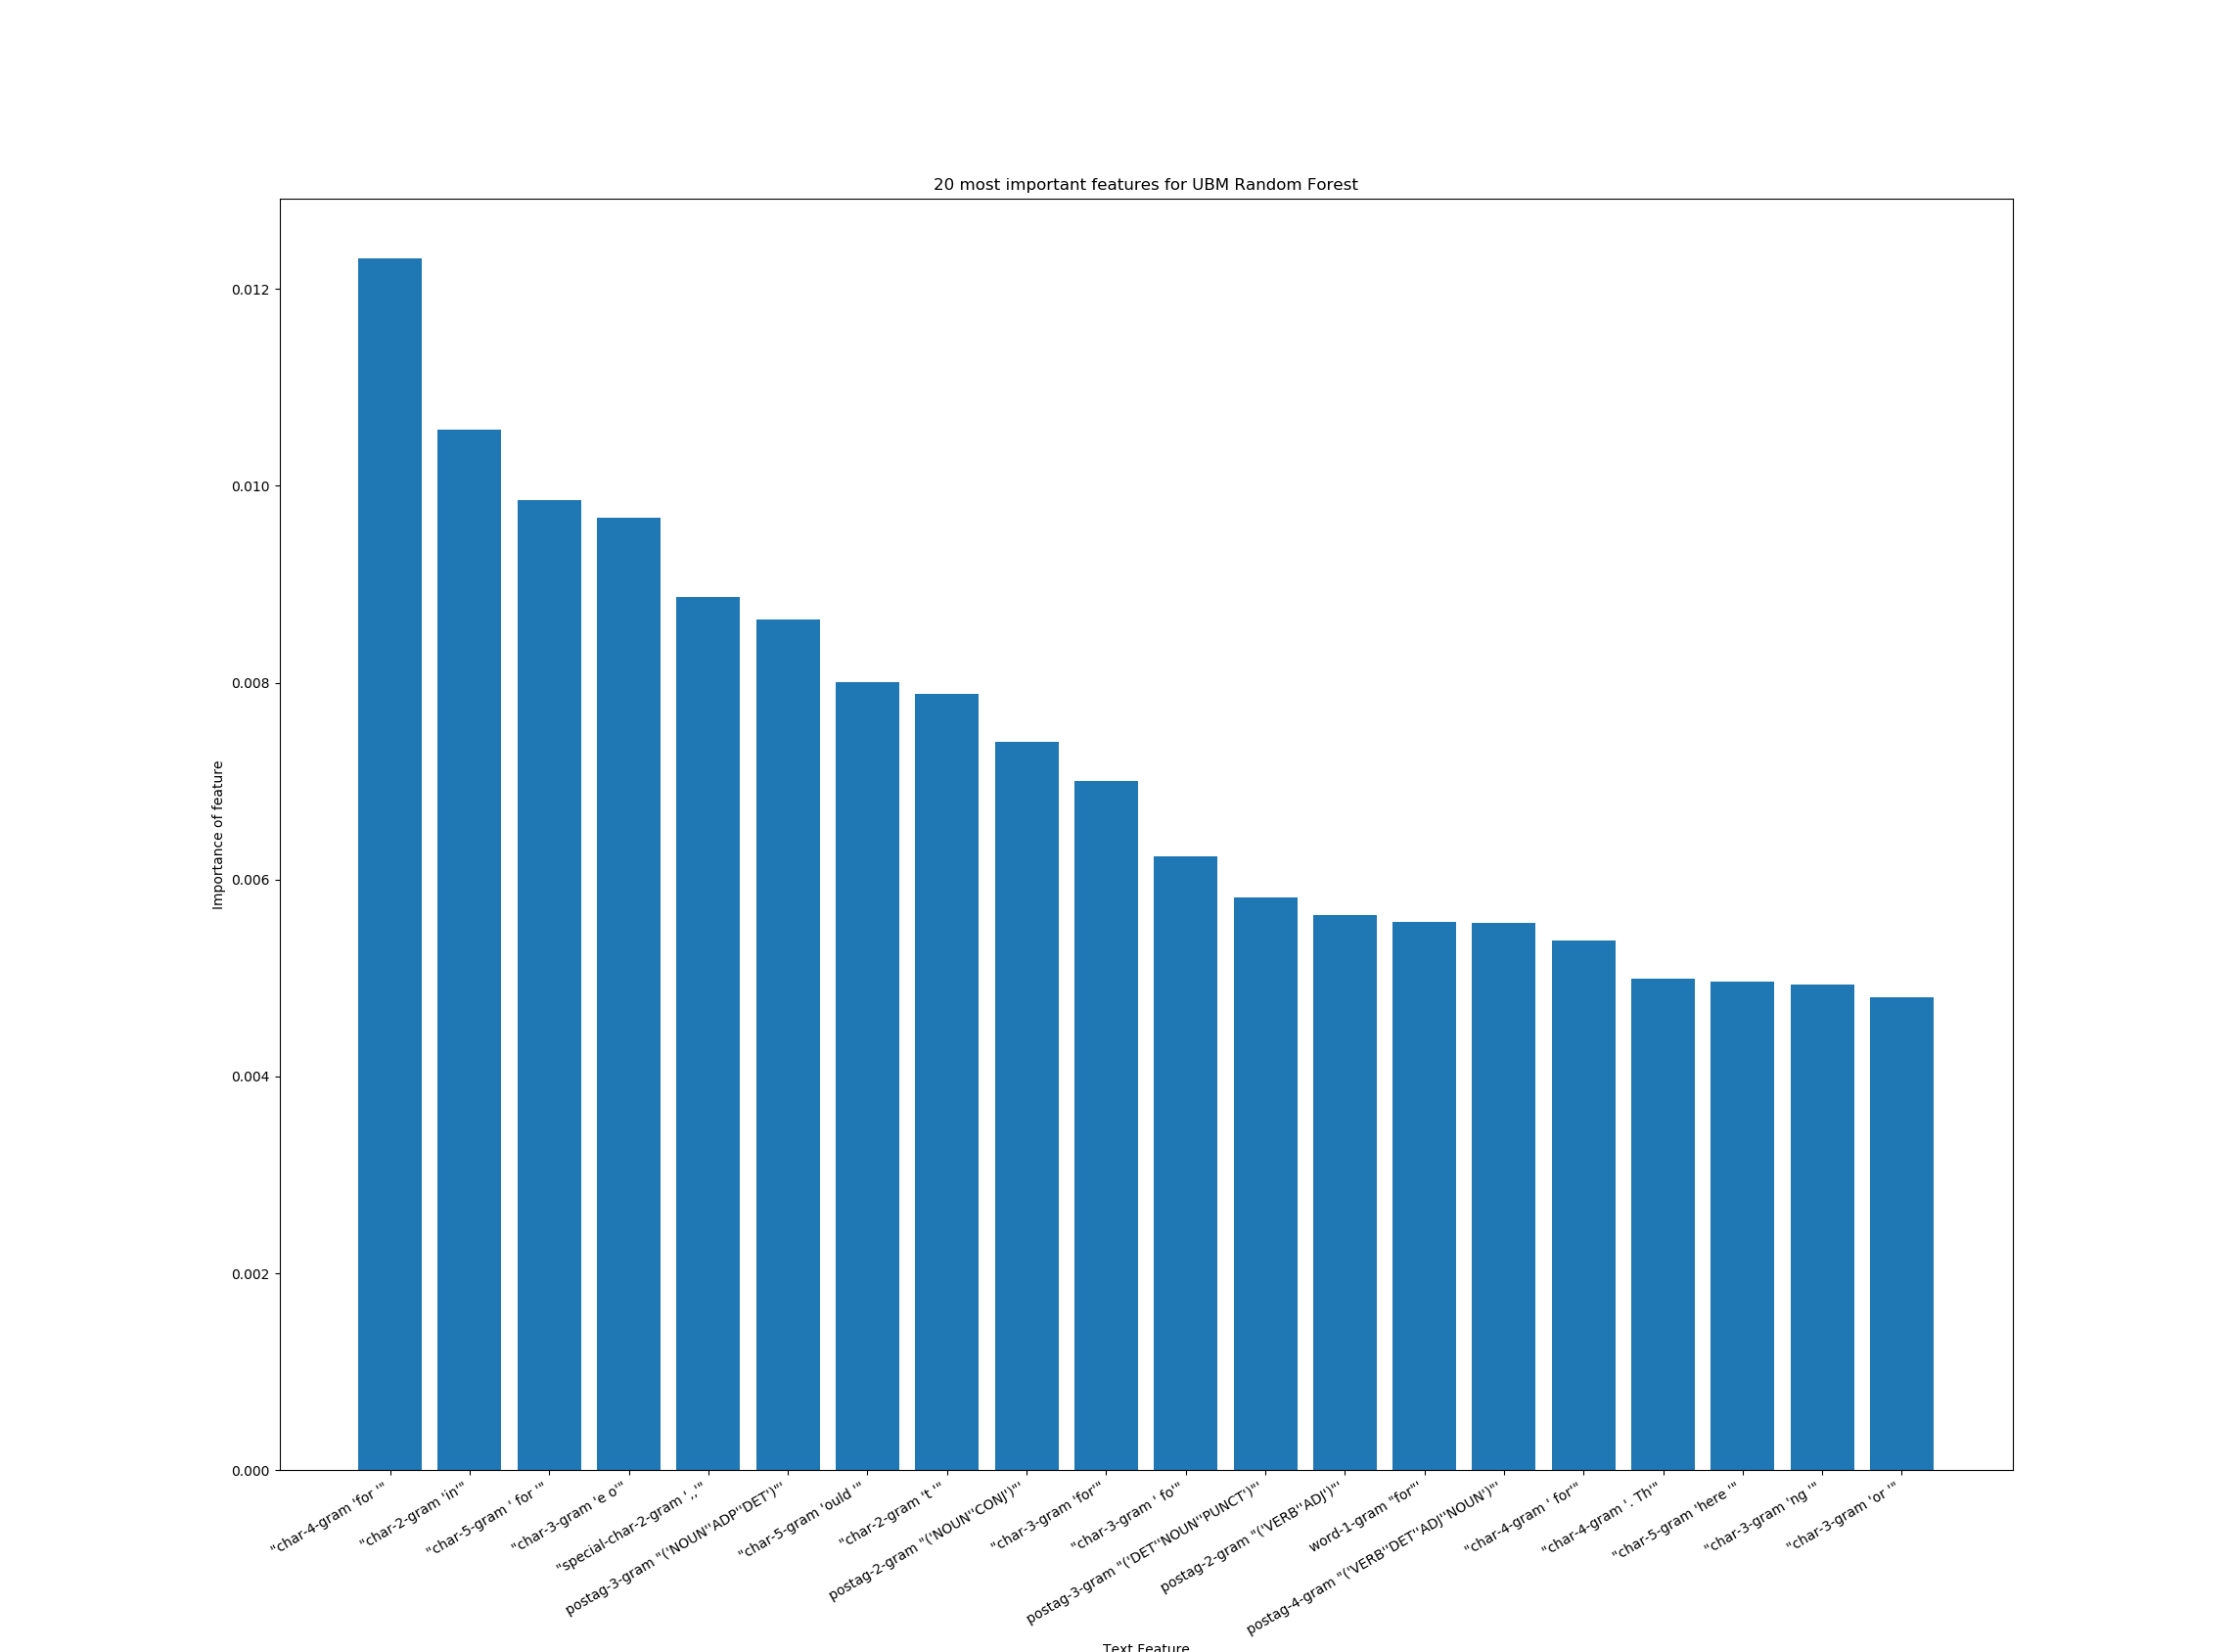
\includegraphics[scale=.34]{./pictures/FeatureImpotrance20.png}
        \caption{The 20 Most important features after applying the UBM encoded
        features to the random forest model}
        \label{fig:feature_importance_small}
    \end{figure}
\end{landscape}

\begin{figure}
    \centering
    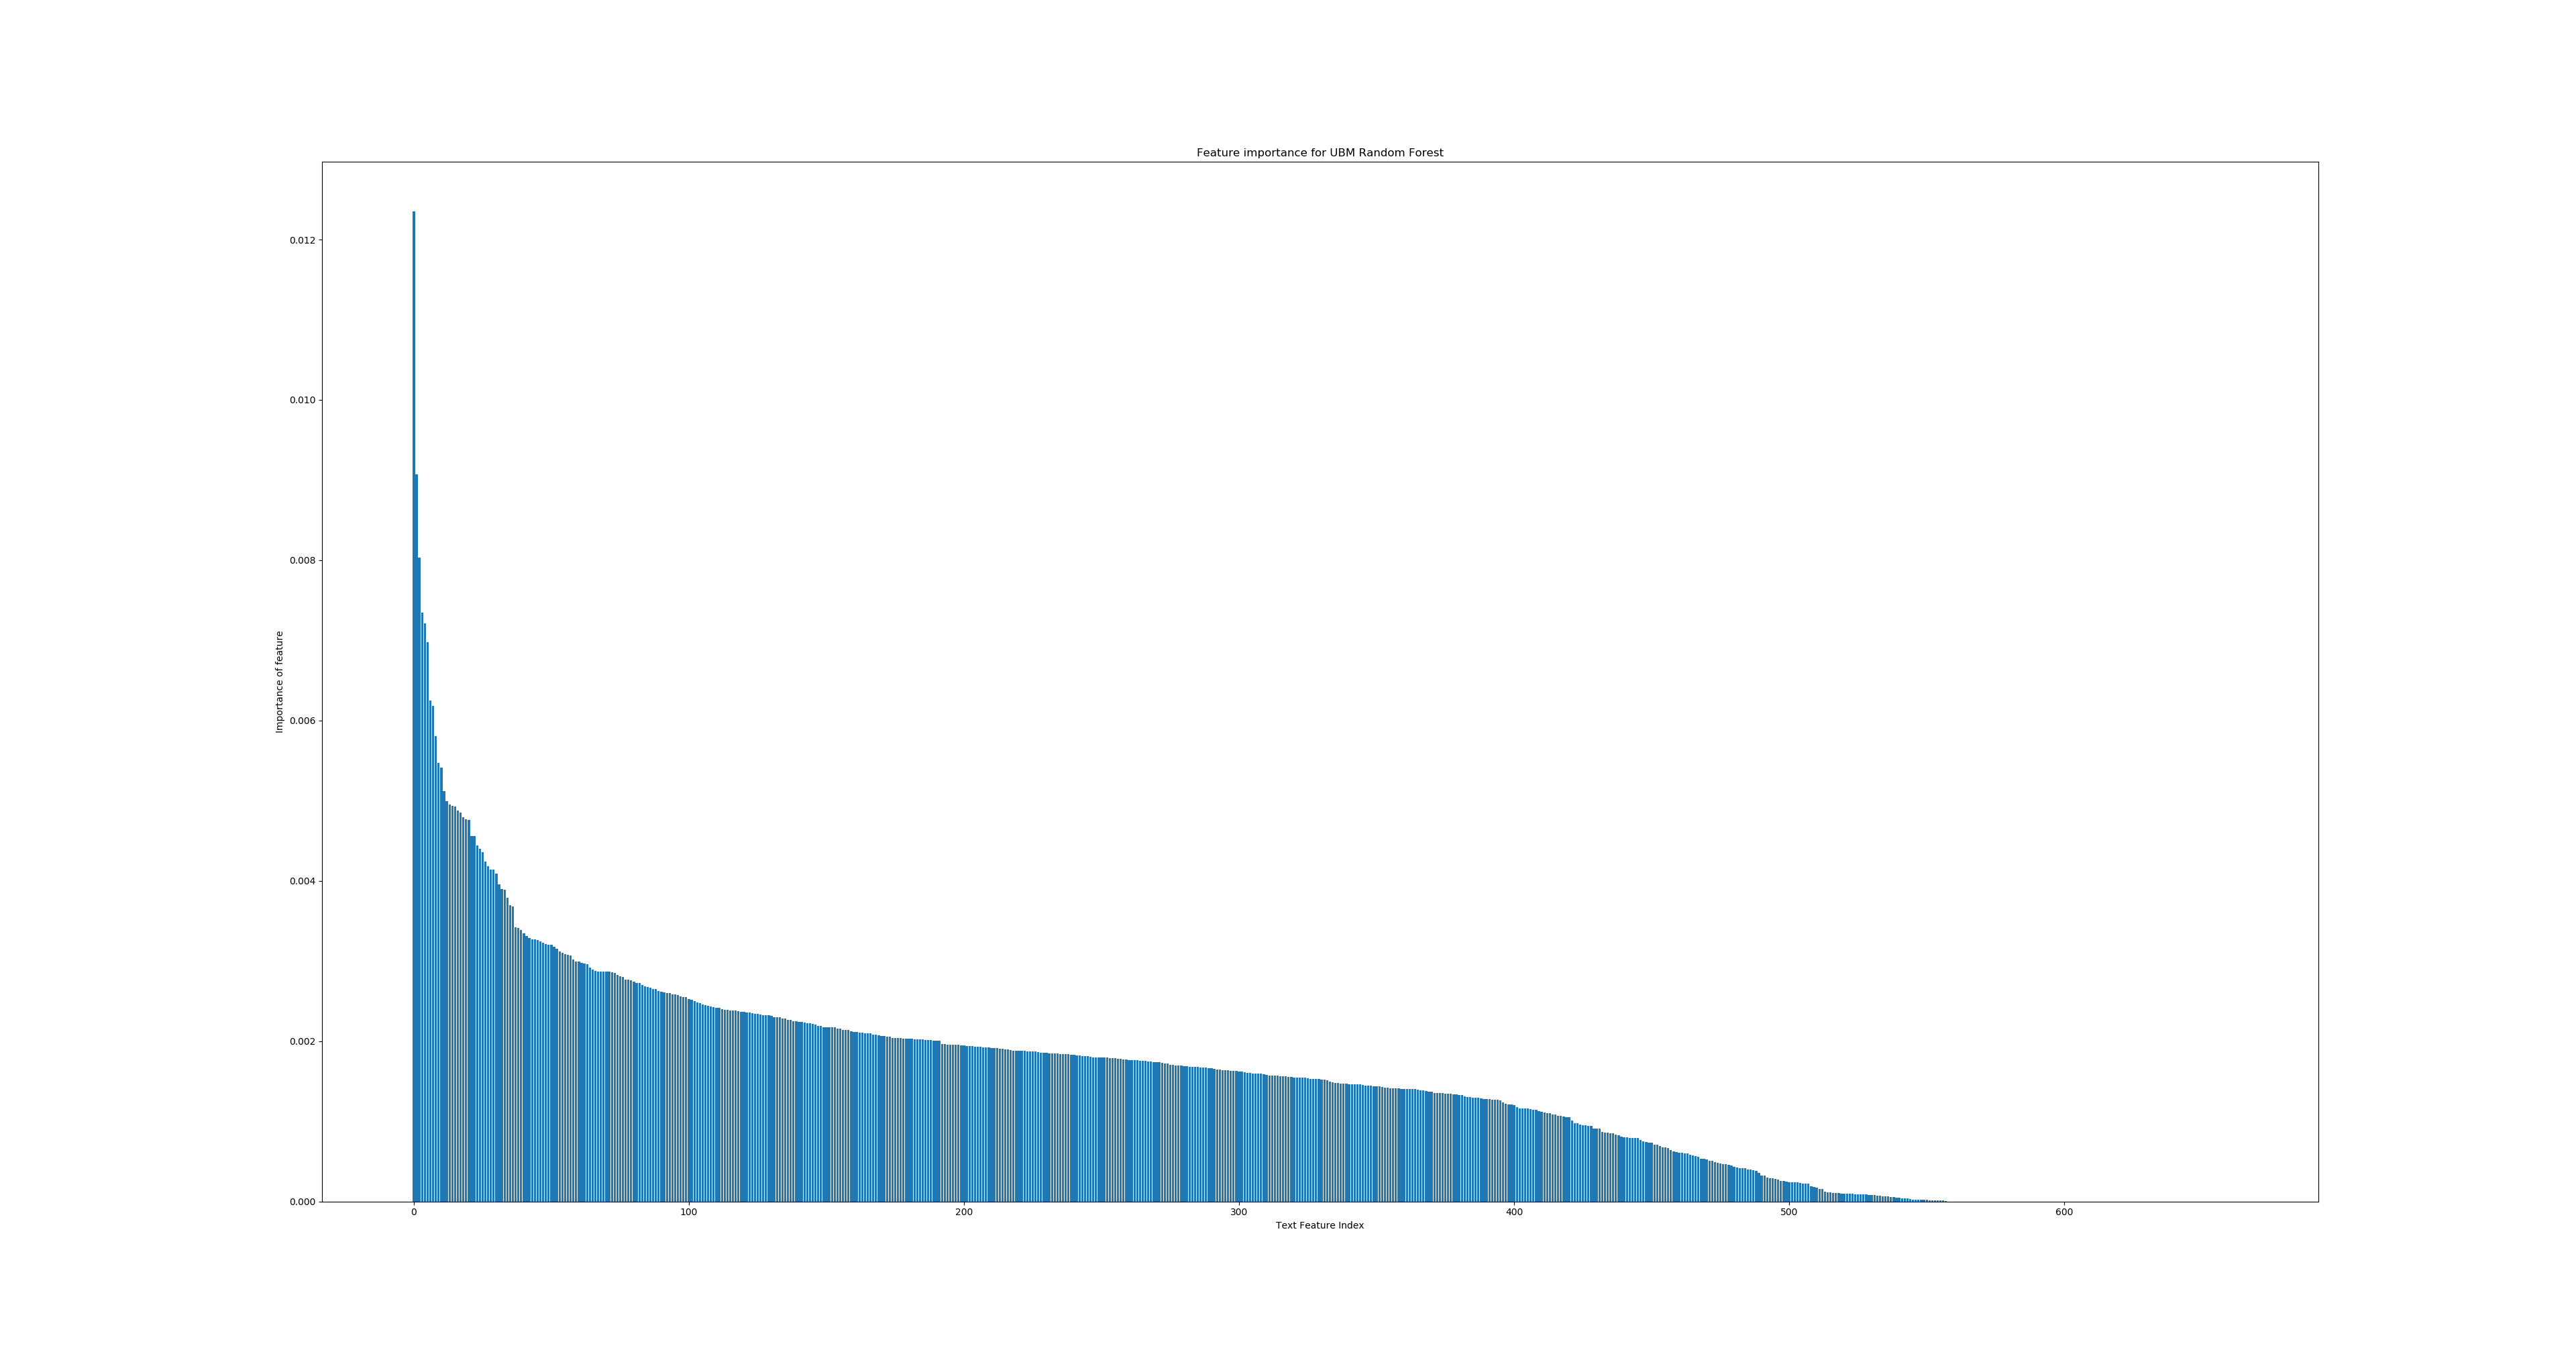
\includegraphics[scale=.34]{./pictures/FeatureImpotranceAll.png}
    \caption{The feature importance for all UBM encoded features given
    to the random forest model}
    \label{fig:feature_importance_all}
\end{figure}

From that overview it is clear that the most important feature is the frequency
of the word \textit{for} as multiple features seem to capture that word. Most
of the words captured by the different features seem to be English stop words.
Both \textit{for}, \textit{in}, \textit{could}, \textit{should}, \textit{would},
\textit{here} and \textit{or} seem to be represented in the list and are part
of the list of English stop words \footnote{https://www.ranks.nl/stopwords}.
Besides that an important feature is the special-character-2-gram consisting
of two commas. That feature might capture an authors prevalence for using long
sentences. Longer sentences will more likely contain a larger amount of commas.
The character-4-gram ". Th" most likely captures an authors tendency to start
her sentences with the word "The". Besides that the \gls{POS}-tags capture the
general sentence structure of the authors.

% TODO: Could we maybe find some article with this point?
The reason the English stop words is so important is probably because they are
consistently used over all genres. Texts about different topics and in different
genres will probably all contain the words \textit{the} and \textit{for}. It is
therefore easier to use them as an estimate of which author has written the text
since they are not dependent on which text the author was writing.

The least important features according to the random forest are shown in Table
\ref{tab:feature_non_importance}. It can be seen that all of those features
consist of word-5-grams and all of them seem to be very specific to a source
text. For example one of the features are the words "in the united states and".
There is a good change that no author will have that phrase at about the same
frequency in all texts she writes. The phrase will clearly be more prevalent in
texts about the United States and less prevalent in cooking recipes even though
they have the same author.

\begin{table}
    \centering
    \begin{tabular}{lll}
        \textbf{Feature Class} & \textbf{Feature} & \textbf{Importance Score} \\
        \hline
        word-5-gram & is one of the most & 0.0 \\
        word-5-gram & index words and electronic switches & 0.0 \\
        word-5-gram & in the united states and & 0.0 \\
        word-5-gram & at the foot of the & 0.0 \\
        word-5-gram & we are born of god & 0.0 \\
        word-5-gram & turned out to be a & 0.0 \\
        word-5-gram & the state of rhode island & 0.0 \\
        word-5-gram & the secretary of the interior & 0.0 \\
        word-5-gram & the second half of the & 0.0 \\
        word-5-gram & the first half of the & 0.0 \\
        word-5-gram & the far end of the & 0.0 \\
        word-5-gram & president of the united states & 0.0 \\
        word-5-gram & of the state of rhode & 0.0 \\
        word-5-gram & of the government of the & 0.0 \\
        word-5-gram & if we are born of & 0.0 \\
        word-5-gram & for the rest of the & 0.0 \\
        word-5-gram & for a number of years & 0.0 \\
        word-5-gram & at the time of the & 0.0 \\
        word-5-gram & are born of god we & 0.0 \\
        word-5-gram & year of our lord one & 0.0
    \end{tabular}
    \caption{The 20 features the random forest least often split on when doing
    authorship verification.}
    \label{tab:feature_non_importance}
\end{table}

It was not only word-5-grams that did not perform very well. After training
our random forest model, it became apparent that there was no case where word
n-grams performed well. The reason for that might be the lack of text in the PAN
2015 dataset. The texts on PAN 2015 being limited to about 150 words meaning
that there are few different word-n-grams in the texts. However, the
word-n-grams extracted from the brown corpus varies a lot and is usually very
subject specific as described above. As such only a few of the word-n-grams
extracted from the brown corpus are in the PAN 2015 texts. This only becomes
more evident as n increases as the word-n-grams becomes more and more text
specific.

Looking at figure \ref{fig:feature_importance_all} however, we can see that
the overall feature contribution is somewhat good. Based on the fact that 600
features were used, meaning that each features importance averages out at
$\frac{1}{600} = 0.00166666666$ if the importance was equally distributed, which
is represented as a line on the graph. As such rather than out model depending
on a very small amount of the total number of features, it can be seen that over
50\% of the feature set actually contributes to the classification. While this
could very well only be the case for out selected features, it does lend some
credence to the idea that using more features in the forest during training
could increase accuracy.

\subsection{Performance of our different methods}
The Delta Method performed better on the training dataset than the testing
dataset. The difference on the PAN 2013 data were 0.06198 and on the PAN 2015
dataset it was 0.03689. It was surprising to us that the performance of the
Delta method deteriorated between train and test since the method does not use
any machine learning. We would have expected the Delta Method to perform the
same on training and testing. The deterioration might be due to the fact that
on both training and testing the Delta Method used the training set for finding
opposing authors. So on training there was a chance that the method would draw
multiple texts from the same author while on test it was guaranteed to only draw
other authors.

The Extended Delta Method achieved the best result of any of our method on the
PAN 2015 data. % TODO: Continues

As for the Generalized Random Forest described in Section
\ref{subsec:method:generalising_random_forest}. This method was off to a bad
start, as the paper it was based on \cite{pacheco2015} only got 6'th place in
the PAN 2015 authorship verification task, and our implementation of that same
method only ranked 9'th. \ref{sec:appendix:pan_2015_results} The main focus of
this method however, was the way it attempted to circumvent the lack of data,
associated with each specific author, by instead learning on the know-text
dataset in its entirety. While the results of this attempt didn't land us at any
place near the top, in terms of placement it did actually work. By comparing out
\gls{UBM} based results to the author specific Minus encoding we can actually
see an improvement in terms of accuracy, thus making the \gls{UBM} a viable
choice when faced with small amounts of entry-specific data.

\subsection{Improvements} 
While the Random Forest method didn't provide any impressive results, the
generalized approach might very well be useful in the future, in case one comes
across another sparse dataset. An improvement that could be done however, was
to increase the number of features fed to the random forest. Not only quantity,
but also different types of features than the ones used in this paper. This
would work since Random Forest by its very nature selects the best features for
classification, we can at the cost of some run time, train on a much larger
feature-set and we suspect better results might be produced, as point supported
by \ref{fig:feature_importance_all} as mentioned earlier.

\begin{itemize}
    \item Why did the delta method perform so much better on the training data?
    \item How does different methods scale to huge amounts of data?
    \item Discuss potential usage in future project based on TPR and TNR.
    \item What improvements could be made to any of the method used. RF Done
    \item Why did SVM's perform so well (https://link.springer.com/article/10.1023/A:1023824908771).
        \begin{itemize}
            \item SVM's can handle many thousands of features.
        \end{itemize}
    \item Manhattan performs better than euclidean in extended delta.
\end{itemize}
